\documentclass[border=4pt]{standalone}
\usepackage{tikz}
\usetikzlibrary{arrows.meta,calc}

\definecolor{orangeText}{HTML}{E3A063}
\definecolor{orangeDim}{HTML}{A87A4E}
\begin{document}
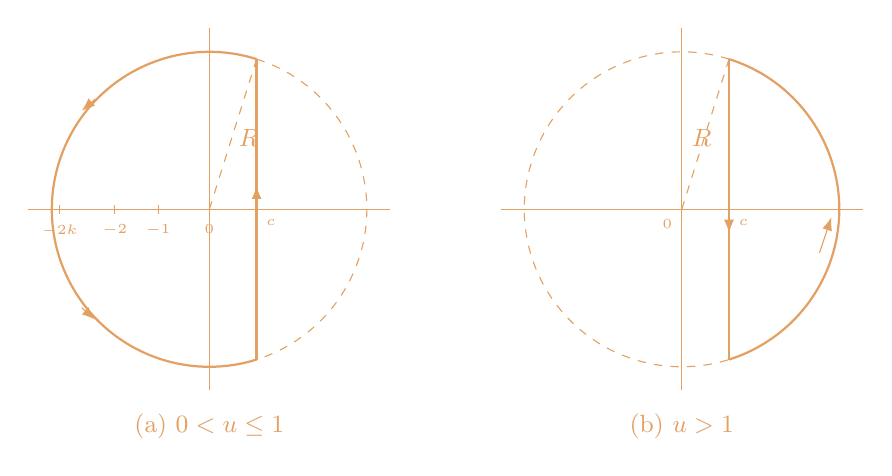
\begin{tikzpicture}[color=orangeText, >=Latex]
    \def\R{2.0}
    \def\c{0.6}
    \pgfmathsetmacro{\h}{sqrt(\R*\R-\c*\c)}
    \pgfmathsetmacro{\ang}{atan2(\h,\c)}

    % ---------- (a) 0 < u <= 1 ----------
    \begin{scope}
        \draw[dashed] (\c,\h) arc (\ang:-\ang:\R);
        \draw[thick] (\c,\h) arc (\ang:360-\ang:\R);
        \draw[thick] (\c,-\h) -- (\c,\h);
        \draw (-2.3,0) -- (2.3,0);
        \draw (0,-2.3) -- (0,2.3);
        \foreach \x/\l in {-1.9/{-2k}, -1.2/{-2}, -0.65/{-1}, 0/0} {
            \draw (\x,-0.06) -- (\x,0.06);
            \node[below] at (\x,-0.07) {\tiny $\l$};
        }
        \node[below right] at (\c,0) {\tiny $c$};
        \draw[dashed] (0,0) -- (\c,\h);
        \node[right] at (0.25,0.9) {\small $R$};
        \draw[-Latex] (\c,-0.3) -- (\c,0.3);
        \draw[-Latex] (-1.45,1.4) -- (-1.62,1.25);
        \draw[-Latex] (-1.62,-1.25) -- (-1.45,-1.4);
        \node at (0,-2.75) {\small (a) $0<u\leq1$};
    \end{scope}

    % ---------- (b) u > 1 ----------
    \begin{scope}[xshift=6cm]
        \draw[dashed] (\c,\h) arc (\ang:360-\ang:\R);
        \draw[thick] (\c,\h) arc (\ang:-\ang:\R);
        \draw[thick] (\c,-\h) -- (\c,\h);
        \draw (-2.3,0) -- (2.3,0);
        \draw (0,-2.3) -- (0,2.3);
        \node[below left] at (0,0) {\tiny $0$};
        \node[below right] at (\c,0) {\tiny $c$};
        \draw[dashed] (0,0) -- (\c,\h);
        \node[left] at (0.5,0.9) {\small $R$};
        \draw[-Latex] (\c,0.3) -- (\c,-0.3);
        \draw[-Latex] (1.75,-0.55) -- (1.9,-0.1);
        \node at (0,-2.75) {\small (b) $u>1$};
    \end{scope}
\end{tikzpicture}
\end{document}
